%%
% Please see https://bitbucket.org/rivanvx/beamer/wiki/Home for obtaining beamer.
%%
\documentclass{beamer}
\usepackage{amsmath,amsbsy,amsopn,amstext,amsfonts,amssymb}
\usepackage{isomath}
\usepackage{ulem}
%\linespread{1.6}  % double spaces lines
\usepackage{graphicx}
\usepackage{subfigure}
\usepackage{color}
\usepackage{optidef}  % define optimization problems
\usepackage{multicol}  % multiple columns
\usepackage{listings} % for python code
\usepackage{mathrsfs}

\usepackage{polynom}
\newcommand{\adj}{\mathrm{adj}}
\newcommand{\constrainedmin}[3]{
		\begin{mini*}|s|
		{#2}{#1}{}{}
		\addConstraint{#3}
		\end{mini*}
}

\newcommand{\rwbcomment}[1]{{\color{blue}RWB:#1}}
\newcommand{\defeq}{\stackrel{\triangle}{=}}
\newcommand{\abs}[1]{\left|#1\right|}
\newcommand{\norm}[1]{\left\|#1\right\|}
\newcommand{\iprod}[1]{\left<#1\right>}
\newcommand{\ellbf}{\boldsymbol{\ell}}
\newcommand{\nubf}{\boldsymbol{\nu}}
\newcommand{\mubf}{\boldsymbol{\mu}}
\newcommand{\abf}{\mathbf{a}}
\newcommand{\bbf}{\mathbf{b}}
\newcommand{\cbf}{\mathbf{c}}
\newcommand{\dbf}{\mathbf{d}}
\newcommand{\ebf}{\mathbf{e}}
\newcommand{\fbf}{\mathbf{f}}
\newcommand{\gbf}{\mathbf{g}}
\newcommand{\hbf}{\mathbf{h}}
\newcommand{\ibf}{\mathbf{i}}
\newcommand{\jbf}{\mathbf{j}}
\newcommand{\kbf}{\mathbf{k}}
\newcommand{\lbf}{\mathbf{l}}
\newcommand{\mbf}{\mathbf{m}}
\newcommand{\nbf}{\mathbf{n}}
\newcommand{\obf}{\mathbf{o}}
\newcommand{\pbf}{\mathbf{p}}
\newcommand{\qbf}{\mathbf{q}}
\newcommand{\rbf}{\mathbf{r}}
\newcommand{\sbf}{\mathbf{s}}
\newcommand{\tbf}{\mathbf{t}}
\newcommand{\ubf}{\mathbf{u}}
\newcommand{\vbf}{\mathbf{v}}
\newcommand{\wbf}{\mathbf{w}}
\newcommand{\xbf}{\mathbf{x}}
\newcommand{\ybf}{\mathbf{y}}
\newcommand{\zbf}{\mathbf{z}}
\newcommand{\Jbf}{\mathbf{J}}
\newcommand{\Acal}{\mathcal{A}}
\newcommand{\Bcal}{\mathcal{B}}
\newcommand{\Lcal}{\mathcal{L}}
\newcommand{\Ncal}{\mathcal{N}}
\newcommand{\Rcal}{\mathcal{R}}
\definecolor{darkolivegreen}{rgb}{0.33, 0.42, 0.18}

\makeatletter
\newenvironment<>{proofstart}[1][\proofname]{%
    \par
    \def\insertproofname{#1\@addpunct{.}}%
    \usebeamertemplate{proof begin}#2}
  {\usebeamertemplate{proof end}}
\newenvironment<>{proofcont}{%
  \setbeamertemplate{proof begin}{\begin{block}{}}
    \par
    \usebeamertemplate{proof begin}}
  {\usebeamertemplate{proof end}}
\newenvironment<>{proofend}{%
    \par
    \pushQED{\qed}
    \setbeamertemplate{proof begin}{\begin{block}{}}
    \usebeamertemplate{proof begin}}
  {\popQED\usebeamertemplate{proof end}}
\makeatother

\title{ECEn 671: Mathematics of Signals and Systems \\ 
Moon: Chapter 3.}
\author{Randal W. Beard}
\institute{Brigham Young University}
\date{\today}

\begin{document}

%-------------------------------
\begin{frame}
	\titlepage
\end{frame}

%-------------------------------
\begin{frame}[t]
\frametitle{Table of Contents}
\tableofcontents
\end{frame}

%%%%%%%%%%%%%%%%%%%%%%%%%%%%%%%%%%%%%%%%%%%%%%%%%%%%%%%%%%%%%%%%%%
\section{Approximation Theory}
\frame{\sectionpage}


%----------------------------------
\begin{frame}\frametitle{Projection and Inner Product}
\begin{itemize}
	\item How does inner product represent a projection?
	
	\item Recall that
	\[ 
	\iprod{ x,y} = \norm{ x }\norm{ y } cos \theta 
	\]
	\begin{center}
	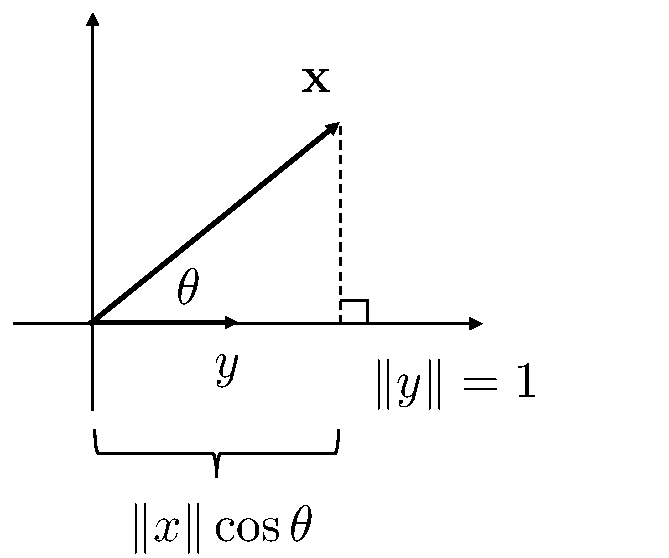
\includegraphics[width=2in]{figures/chap3_projection}
	\end{center}
	
	\item In 2-D $\iprod{ x,y}$ represents the length of the projection of $x$ in the direction of $y$.

	\item In general, inner products represent (non-orthogonal) projection of one vector onto another.
\end{itemize}
\end{frame}


%----------------------------------
\begin{frame}\frametitle{Approximation Problem}
	\begin{itemize}
	\item Let $\mathbb{S}$ be a Hilbert space, and let $x \in \mathbb{S}$.

	\item Let $\{p_1, \dots, p_n \}$ be a set of vectors, all in $\mathbb{S}$.
	\item Find $\hat{x} \in \text{span}\{ p_1, \ldots p_n \}$ that minimizes $\norm{x-\hat{x}}$.
	\end{itemize}
\end{frame}

%----------------------------------
\begin{frame}\frametitle{Approximation Problem, cont}
	\begin{itemize}
	
	\item Let $\hat{x} = c_1 p_1 + \ldots + c_n p_n \in \text{span}\{p_1, \dots, p_n\}$.
	\item By the projection theorem, the error
	\begin{align*}
		e &= x - \hat x \\
		  &= x - c_1 p_1 - \ldots - c_n p_n
	\end{align*}
	is minimized if 
	\[
	e \perp \text{span}\{ p_1, \ldots, p_n\}.
	\]
	\end{itemize}
\end{frame}

%----------------------------------
\begin{frame}\frametitle{Approximation Problem, cont}
	\[
	e \perp \text{span}\{ p_1, \ldots, p_n\}.
	\]
	iff
	\begin{align*}
		\iprod{ e, p_1} &= 0\\
		\iprod{ e, p_2} &= 0\\
		\vdots\\
		\iprod{ e, p_n } &= 0	
	\end{align*}
	iff
	\begin{align*}
		\iprod{ x - c_1p_1 - \ldots c_np_n, p_1 } &= 0\\
		\vdots\\
		\iprod{ x - c_1p_1 - \ldots c_np_n, p_n } &= 0
	\end{align*}
\end{frame}

%----------------------------------
\begin{frame}\frametitle{Approximation Problem, cont}
	By properties of the inner product we can write this as
	\begin{flalign*}
	\iprod{ x,p_1 } - c_1 \iprod{ p_1, p_1} - \cdots - c_n \iprod{ p_n, p_1} &= 0\\
	\vdots\\
	\iprod{ x,p_n} - c_1 \iprod{ p_1,p_n} - \cdots - c_n \iprod{ p_n, p_n} &= 0
	\end{flalign*}
	or in matrix notation,
	\[
	\underbrace{
		\left(
		\begin{array}{ccc}
		\iprod{ p_1, p_1} & \cdots & \iprod{ p_n, p_1}\\
		\vdots & & \vdots \\
		\iprod{ p_1, p_n} & \cdots & \iprod{ p_n, p_n}
		\end{array}
		\right)
	}_{R}
	\underbrace{\left(
	\begin{array}{c}
	c_1\\
	\vdots\\
	c_n
	\end{array}
	\right)}_{\cbf}
	= 
	\underbrace{\left(
	\begin{array}{c}
	\iprod{ x, p_1}\\
	\vdots\\
	\iprod{ x, p_n}
	\end{array}
	\right)}_{\pbf}
	\]
	$R$ is called the Grammian of the set $\{p_1,\ldots,p_n\}$.
\end{frame}

%----------------------------------
\begin{frame}\frametitle{The Grammian of a set}
	\begin{definition}[Grammian]
	Given a set $\{p_1, \dots, p_n\}$ of vectors in $\mathbb{S}$, the \underline{Grammian} of the set is the matrix
	\[
	R = \begin{pmatrix}
 			\iprod{ p_1, p_1} & \cdots & \iprod{ p_n, p_1}\\
			\vdots & & \vdots \\
			\iprod{ p_1, p_n} & \cdots & \iprod{ p_n, p_n}
 		\end{pmatrix}
	\]	
	\end{definition}
	
	\par\noindent Note that $R^H = R$
	
	\par\noindent We also have the following theorem:
	
	\begin{theorem}[Moon, Theorem 3.1]
	The Grammian $R$ is positive definite iff the set of vectors 
	$\{p_1,\ldots p_n\}$ are linearly independent.
	\end{theorem}
\end{frame}

%----------------------------------
\begin{frame}\frametitle{Proof}
	Let $y \in \mathbb{S}$ then 
	\begin{flalign*}
	y^H R y &= (\bar{y}_1 \cdots \bar{y}_n) 
	\left(
	\begin{array}{ccc}
	\iprod{ p_1, p_1 } & \ldots & \iprod{ p_n,p_1}\\
	\vdots &  & \vdots \\
	\iprod{ p_1,p_n} & \ldots & \iprod{ p_n, p_n }
	\end{array}
	\right)
	\left(
	\begin{array}{c}
	y_1\\
	\vdots\\
	y_n
	\end{array}
	\right)\\
	&= \left( \sum_{i=1}^n \bar{y}_i\iprod{ p_1,p_i} \ldots
	\bar{y}_i\sum_{i=1}^n \iprod{ p_n,p_i} \right)
	\left( \begin{array}{c}
	y_1\\
	\vdots\\
	y_n
	\end{array}
	\right)\\
	&= \sum_{j=1}^n \sum_{i=1}^n \bar{y}_iy_j \iprod{ p_j, p_i}\\
	&= \iprod{ \sum y_jp_j, \sum y_i,p_i} = \parallel \sum y_i
	p_i \parallel^2 \geq 0
	\end{flalign*}
	Therefore $R$ is always positive semi-definite.
\end{frame}

%----------------------------------
\begin{frame}\frametitle{Proof, cont.}
\begin{description}
\item[($\Rightarrow$):]
	Suppose that $R$ is pd then
	\begin{flalign*}
	y^HRy &= \norm{ \sum y_ip_i }^2 > 0\\
	&\Rightarrow \sum y_i p_i \neq 0 \text{ for all nonzero $y \in \mathbb{S}$}\\
	&\Rightarrow \{p_1,\cdots p_n\} \text{ is linearly independent}
	\end{flalign*}

\item[($\Leftarrow$):]	
	Conversely suppose $\{p_1, \cdots p_n\}$ is linearly independent, but
	$R$ is only psd.  $R$ is psd implies that $\exists y \neq 0$ such that 
	\begin{align*} 
		& y^HRy = \norm{ \sum y_ip_i }^2 = 0 \\
		\Rightarrow & \sum y_ip_i = 0 \\ 
		\Rightarrow & \{p_1, \cdots p_n\} \text{is linearly dependent.}
	\end{align*}
	Which contradicts the assumption that R is psd.
\end{description}
\end{frame}

%----------------------------------
\begin{frame}\frametitle{Orthogonality Theorem}
	\begin{theorem}[Moon, Theorem 3.2]	
	Let $p_1,p_2, \cdots p_n $ be data vectors (or basis vectors) in a
	Hilbert space $\mathbb{S}$.  Let $x \in \mathbb{S}$.  Let $e$ be defined as
	\[ e \defeq x - \hat{x} = x - \sum_{j=1}^n c_j p_j,\]
	then $e$ is minimized when it is orthogonal to each of the data
	vectors, i.e.
	\[ \iprod{ e, p_j} = 0 \qquad j=1,\ldots, n \]
	Equivalently
	\[
	R\cbf = \pbf.
	\]
	\end{theorem}
	\begin{proof}
		Follows directly from projection theorem.
	\end{proof}
\end{frame}

%----------------------------------
\begin{frame}\frametitle{Calculus-Based Approach (Alternative proof)}
	Rather than using the projection theorem, we can derive the same result using calculus.
	
	\vfill
	
	\par\noindent{\bf Problem Statement:}
	Let $\ebf = x - \sum_{i=1}^n c_i p_i$.  Find $\cbf=(c_1, \dots, c_n)^\top$ that minimizes $\norm{\ebf}$.
	
	\vfill
	
	\par\noindent{\bf Solution:}
	First note that minimizing $\norm{\ebf}^2$ is equivalent to minimizing $\norm{e}$.
	Also note that 
	\begin{align*}
	\norm{e}^2 &= \iprod{ x - \sum c_jp_j, x - \sum c_j p_j}\\
		&= \norm{x}^2 - 2 Re\{ \sum_{i=1}^n \bar{c}_i\iprod{
			x,p_i}\} + \sum \sum c_j \bar{c}_i \iprod{ p_j, p_i}	 \\
		&= \norm{x}^2 - 2 Re\{ \cbf^H\pbf \} +\cbf^H R \cbf.
	\end{align*}
	
\end{frame}

%----------------------------------
\begin{frame}\frametitle{Calculus-Based Approach, cont.}

	To minimize 
	\[
	\norm{e}^2 = \norm{x}^2 - 2 Re\{ \cbf^H\pbf \} +\cbf^H R \cbf
	\]
	differentiate with respect to $\cbf$ and set to zero.  This
	will be a local minima if the second derivative is psd.
\end{frame}

%----------------------------------
\begin{frame}\frametitle{Calculus-Based Approach, cont.}
	From Moon Appendix we have
	\begin{align*}
	\frac{\partial}{\partial \bar{\cbf}} Re\{\cbf^H \pbf\} &= \frac{1}{2}\pbf \\
	\frac{\partial}{\partial \bar{\cbf}} \cbf^H R \cbf &= R\cbf
	\end{align*}
	Therefore
	\[ 
	\frac{\partial \norm{e}^2}{\partial \bar{\cbf}} = -\pbf + 
	R \cbf = 0 \qquad \Rightarrow \qquad R \cbf = \pbf 
	\]
	In addition, we have that
	\[ 
	\frac{\partial^2 \norm{e}^2}{\partial \bar{\cbf}} = R \geq 0.
	\]
	Therefore the solution of $R\cbf=\pbf$ minimize $\norm{e}$.
	
	$R\cbf = \pbf$ is the same equation we obtained using the
	projection theorem.
	
\end{frame}

%----------------------------------
\begin{frame}\frametitle{Matrix Representation}
	\begin{itemize}
	\item 	Stack the vectors $\{ p_1, \ldots p_n\}$ in a matrix
	\begin{align*}
	A &= \begin{pmatrix}p_1 & p_2 & \ldots & p_n \end{pmatrix} \\
 	\cbf &= \begin{pmatrix} c_1 & c_2 & \ldots & c_n \end{pmatrix}^\top	
	\end{align*}
	
	\item Then $\hat{x} = \sum c_j p_j = A \cbf$.
	\item Therefore $\ebf = x - \hat{x} = x - A\cbf$.
	\end{itemize}
\end{frame}

%----------------------------------
\begin{frame}\frametitle{Matrix Representation, cont.}
	\begin{itemize}
	\item Project $\ebf$ onto $\{p_1 \ldots p_n\}$:
		\begin{align*}
		\iprod{ x-A\cbf, p_1} &= p_1^H (x-A\cbf) = 0\\
		\vdots\\
		\iprod{ x-A\cbf, p_n} &= p_n^H (x - A \cbf) = 0
		\end{align*}
		
	\item Note that $A^H = \left[ \begin{array}{c} p_1^H \\ \vdots \\
	p_n^H \end{array} \right]$.
	
	\item Rewrite as
	\begin{align*}
	& A^H(x-A\cbf) = 0 \\
	\Rightarrow & \underbrace{A^HA}_{R}\cbf = \underbrace{A^Hx}_{\pbf}
	\end{align*}
	\end{itemize}
\end{frame}

%----------------------------------
\begin{frame}\frametitle{Matrix Representation, cont.}
	\begin{itemize}	
	\item If $\{p_1, \ldots p_n\}$ are linearly independent then $R > 0$ which implies that $R^{-1}$ exists, so
	\[ \cbf = (A^HA)^{-1}A^Hx \]

	\item Since $\hat{x} = A\cbf$ we have that
	\[
	\hat{x} = A (A^H A)^{-1} A^H x
	\]
	is the best approximation to $x$ in $\text{span}\{p_1, \dots, p_n\}$.
	
	\item {\bf Fact:}  $P_A = A(A^HA)^{-1}A^H$ is a projection operator from $S$ to $span\{p_1,\ldots,p_n\}$
	\end{itemize}
\end{frame}

%----------------------------------
\begin{frame}\frametitle{Application:Polynomial Approximation}
	\begin{itemize}
	\item Suppose you are given a real continuous function $f(t)$ and you would like to approximate it by an $m^{th}$ order polynomial on the interval $[a,b]$.
	\item Let the basis vectors be $\{1,t,\ldots,t^m\}$.
	\item Then $\hat{f}(t) = c_1 + c_2t + \cdots + c_{m+1} t^m$
	\item Define the inner product as $\iprod{ f,g} = \displaystyle
	\int_{a}^{b} f(t)g(t) dt$
	\end{itemize}
\end{frame}

%----------------------------------
\begin{frame}\frametitle{Application: Polynomial Approximation, cont.}	
	
	Then the orthogonality theorem implies that the ``best'' approximation is
	given by 
	\begin{align*}
	\iprod{ f - \hat{f}, 1} &= 0\\
	\vdots\\
	\iprod{ f - \hat{f}, t^m } &= 0
	\end{align*}
	or
	\[
	\underbrace{
		\left( \begin{array}{ccc}
		\iprod{ 1,1 } & \cdots & \iprod{ t^m, 1}\\
		\vdots & & \vdots \\
		\iprod{ 1,t^m} & \cdots & \iprod{ t^m, t^m }
		\end{array}
		\right)}_{\text{ Grammian Matrix }}
	\left(
	\begin{array}{c}
	c_1\\
	\vdots\\
	c_{m+1}
	\end{array}
	\right)
	=
	\left( \begin{array}{c}
	\iprod{ f,1 }\\
	\vdots\\
	\iprod{ f, t^m }
	\end{array}
	\right)
	\]	
	or
	\[ R \cbf = \pbf.  \]
\end{frame}

%----------------------------------
\begin{frame}\frametitle{Application: Linear Regression}
	\begin{itemize}
	\item Suppose you have a number of data points that you are trying to fit to a line.
		\begin{center}
		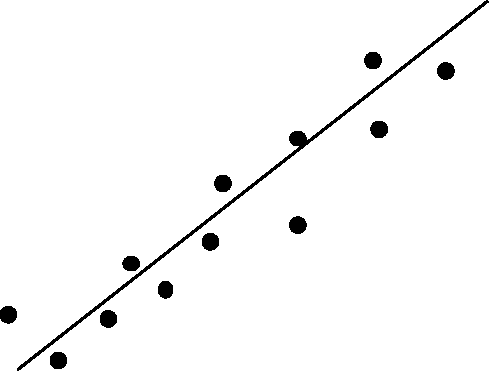
\includegraphics[width=1.5in]{figures/chap3_linear_regression}
		\end{center}
		
	\item Given $(x_i, y_i) \qquad i = 1,\ldots N$
	
	\item The equation for a line is $y = ax + b$
	\item {\bf Problem:}  Find $a$ and $b$ that minimizes the mean squared error $\sum_{i=1}^N \abs{y_i - ax_i - b}^2$
	\end{itemize}	
\end{frame}
 
%----------------------------------
\begin{frame}\frametitle{Application: Linear Regression, cont.}	
	\begin{itemize}
	\item For each data point we have
	\[ e_i = y_i - ax_i - b \]
	where $e_i$ is the error for the $i^{th}$ data point.  
	
	\item Let
	\[ \ybf = \left( \begin{array}{c} y_1\\ \vdots \\ y_N \end{array}
	\right), \quad 
	\ebf = \left( \begin{array}{c} e_1 \\ \vdots \\
	e_N \end{array} \right), \quad
	A = \left( \begin{array}{cc} x_1 & 1
	\\ \vdots & \vdots \\ x_N & 1 \end{array} \right), \quad
	\cbf
	= \left( \begin{array}{c} a \\ b \end{array} \right) \]
	
	\item Then $\ebf = \ybf-A\cbf$.
	\end{itemize}	
\end{frame}
 
%----------------------------------
\begin{frame}\frametitle{Application: Linear Regression, cont.}	
	\begin{itemize}
	\item Project the error $\ebf$ on the data vector (columns of $A$) and set to zero:
	\[
	A^H \ebf = A^H (\ybf - A\cbf) =0
	\]
	
	\item Therefore
	\[ A^H A \cbf = A^H \ybf \]
	
	\item Giving the minimum least squares solution
	\[ \cbf = (A^H A)^{-1} A^H \ybf. \]
	
	\end{itemize}	
\end{frame}


%%%%%%%%%%%%%%%%%%%%%%%%%%%%%%%%%%%%%%%%%%%%%%%%%%%%%%%%%%%%%%%%%%
\section{Dual Approximation}
\frame{\sectionpage}

%----------------------------------
\begin{frame}\frametitle{Dual Approximation}
	This section develops an approach that allows approximation in infinite dimensional spaces with finite constraints.
	
	\vfill
	
	For matrices, we will solve the problem
	\begin{mini*}|s|
	{}{\norm{x}}{}{}
	\addConstraint{Ax = b}	
	\end{mini*}
\end{frame}

%----------------------------------
\begin{frame}\frametitle{Dual Approximation, cont.}
\begin{definition}[Affine Space]
	Let $\mathbb{Y}$ be a subspace of $\mathbb{S}$ and let $x_o \in \mathbb{S}$.  The set $\mathbb{V} = x_0 + \mathbb{Y}$ is called a \underline{linear variety} or an \underline{affine} space.
	\begin{center}
	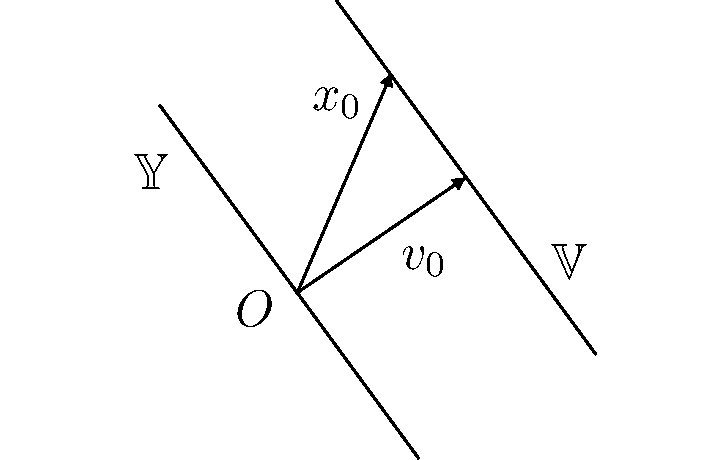
\includegraphics[width=2in]{figures/chap3_affine_space}
	\end{center}
\end{definition}
	
	The projection theorem says that there exists a $v_0 \in \mathbb{V}$ such that
	$v_0 = \underset{v \in \mathbb{V}}{\arg\min}\norm{ v }$ such that
	$v_0 \perp \mathbb{Y}$.

\end{frame}

%----------------------------------
\begin{frame}\frametitle{Dual Approximation, cont.}
	Let $M = span\{y_1, \ldots, y_m\}$ then $\text{dim}(M) < \infty$.
	
	\vfill
	
	If $\text{dim}(\mathbb{S}) = \infty$ then $\text{dim}(M^{\perp}) = \infty$ where $M^{\perp}$ is the set of all $x \in \mathbb{S}$ such that
	\begin{align*}
	\iprod{x, y_1} &= 0 \\
	\vdots \\
	\iprod{x, y_m} &=0	
	\end{align*}
\end{frame}

%----------------------------------
\begin{frame}\frametitle{Dual Approximation, cont.}	

	Now suppose that there are $m$ inner product constraints:
	\begin{align*}
	\iprod{ x, y_1} &= a_1\\
	\vdots\\
	\iprod{ x, y_m} &= a_n
	\end{align*}
	If $\exists x_0$ that satisfies the constraints then so does $x_0 + v$ where $v \in M^{\perp}$ since
	\begin{align*}
	\iprod{ x_0+v, y_j} &= \iprod{ x_0, y_j} + \iprod{v, y_j} \\
						&= \iprod{ x_0,y_j} \\
						&= a_j 
	\end{align*}
	
	Therefore all solutions are in the (infinite dimensional) affine space
	\[ v = x_0 + M^{\perp} \]
	
\end{frame}

%----------------------------------
\begin{frame}\frametitle{Dual Approximation, cont.}	
	\begin{theorem}[Moon Theorem 3.4]
		Let $\{ y_1, \cdots, y_m\} $ be linearly independent in a Hilbert
		space $\mathbb{S}$, and let $M = span\{y_1, \cdots, y_m\}$.	
		The solution of the problem
		\begin{mini*}|s|
		{x\in \mathbb{S}}{\norm{x}^2}{}{}
		\addConstraint{\iprod{x, y_1} &= \alpha_1}	
		\addConstraint{\vdots}
		\addConstraint{\iprod{x, y_m} &= \alpha_m}
		\end{mini*}
		is an element of $M$, i.e., $\hat{x} = \arg\min_{x\in\mathbb{S}}\norm{x}^2 = \sum_{i=1}^{m} c_i y_i$,
		where $\cbf$ satisfies $R\cbf = \boldsymbol{\alpha}$, where $R$ is the Grammian and 
		\[
			\boldsymbol{\alpha} = (\alpha_1, \dots, \alpha_m)^\top.
		\]
	\end{theorem}
	
\end{frame}

%----------------------------------
\begin{frame}\frametitle{Proof:}
	From the previous discussion, the solution lies in the affine space  $\mathbb{V} = x_0 + M^{\perp}$ for some $x_0 \in \mathbb{S}$.
	\begin{center}
	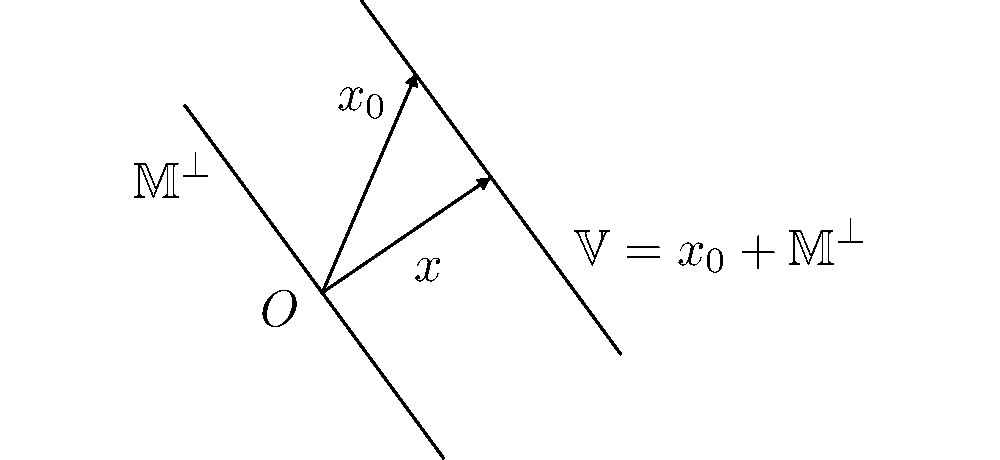
\includegraphics[width=3in]{figures/chap3_dual_approximation}
	\end{center}

	\vfill
	
	The minimum norm solution is orthogonal to $M^{\perp}$ i.e. $\hat{x} \perp
	M^{\perp} \Rightarrow \hat{x} \in M^{\perp \perp} = M$

	\vfill
	
	So $\hat{x}$ is of the form $\hat{x} = \displaystyle \sum_{j=1}^{m}c_jy_j$
\end{frame}

%----------------------------------
\begin{frame}\frametitle{Proof, cont.}
	Now projecting $x$ onto $M$ gives
	\begin{align*}
	\iprod{ \hat{x},y_1} &= \iprod{ \sum c_jy_j, y_1} &= \sum c_j
	\iprod{ y_j, y_1} &= \alpha_1 \\
	\vdots\quad &= \qquad\vdots\qquad &= \qquad\vdots\qquad &= ~~\vdots\\
	\iprod{ \hat{x},y_m} &= \iprod{ \sum c_j y_j, y_m} &= \sum c_j
	\iprod{ y_j,y_m} &= \alpha_m
	\end{align*}
	rewriting in matrix notation gives
	\[ R\cbf = \boldsymbol{\alpha} \]	
\end{frame}


%----------------------------------
\begin{frame}\frametitle{Dual Approximation, Example}
	Given the differential equation
	\[ 
	\ddot{y} + 6\dot{y} + 8y = 4\dot{u} + 10u, \qquad y(0)=\dot{y}(0) =0 
	\]
	Solve the following optimal control problem:
		\begin{mini*}|s|
		{u\in L_2}{\norm{u}^2}{}{}
		\addConstraint{y(1) = 1}	
		\addConstraint{\int_0^1 y(t)dt &= 0}
		\end{mini*}
\end{frame}

%----------------------------------
\begin{frame}\frametitle{Dual Approximation, Example, cont.}
	The corresponding transfer function is
	\begin{align*}
	& H(s) = \frac{4s + 10}{s^2 + 6s + 8} = \frac{1}{s+2} + \frac{3}{s+4} \\
	\Rightarrow & h(t) = e^{-2t} + 3e^{-4t} \\
	\Rightarrow & y(t) = \int_0^t\left[e^{-2(t-\tau)} + 3e^{-4(t-\tau)}\right]u(\tau) d\tau 
	\end{align*}
	
	\vfill
	
	Define the following inner product
	\[ 
	\iprod{f(t), g(t)} = \int_0^1 f(\tau)g(\tau)d\tau 
	\]
	then $y(1) = 1$ can be written as
	\[ \int_0^1 \left[ e^{-2(1-\tau)} + 3e^{-4(1-\tau)}\right]u(\tau)d\tau =
	\iprod{ u,y_1} = 1 \]
	where $y_1(t) = e^{-1(1-t)}+3e^{-4(1-t)}$
\end{frame}

%----------------------------------
\begin{frame}\frametitle{Dual Approximation, Example, cont.}
	The second constraint is of the form 
	\[ \int_0^1 y(t)dt = \int_{t=0}^{t=1} \int_{\tau = 0}^{\tau = t}h(t -
	\tau)u(\tau)d\tau dt = 0 \]
	
	\begin{center}
	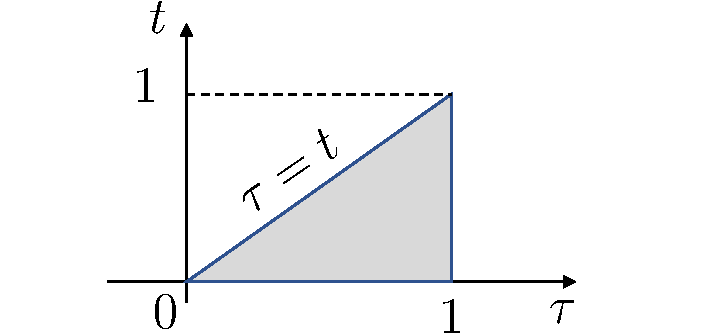
\includegraphics[width=5cm]{figures/chap3_change_of_variables}
	\end{center}
	
	Changing order of integration gives
	\[ = \int_{\tau = 0}^{1}\left[\int_{t = \tau}^{1}
	h(t-\tau)dt\right]u(\tau)d\tau. \]

\end{frame}

%----------------------------------
\begin{frame}\frametitle{Dual Approximation, Example, cont.}	
	Letting $\sigma = t - \tau \Rightarrow t = \sigma + \tau \Rightarrow
	dt = d\sigma$ gives
	\[ = \int_{\tau = 0}^{1} \left[ \int_{\sigma=0}^{\sigma=1-\tau}
	h(\sigma)d\sigma \right] u(\tau) d\tau \]
	\[ = \int_{\tau = 0}^{1}\left( \frac{5}{4} -
	\frac{3}{4}e^{-4(1-\tau)}-\frac{1}{2}e^{-2(1-\tau)}\right)u(\tau)d\tau \]
	\[ = \iprod{u,y_2 } = 0\]
	where 
	\[y_2(t) = \frac{5}{4} -\frac{3}{4}e^{-4(1-\tau)}-\frac{1}{2}e^{-2(1-\tau)} \]
	so we have that 
	\begin{align*}
	\iprod{u,y_1 } &= 1\\
	\iprod{u,y_2 }&= 0
	\end{align*}
	and we want to minimize $\norm{u }^2_{L_2[0,1]}$
\end{frame}
	
%----------------------------------
\begin{frame}\frametitle{Dual Approximation, Example, cont.}	
		
	Let $M = span\{y_1,y_2\}$.

	By Theorem 3.4 
	\[ 
	u \in M \Rightarrow u(t) = c_1y_1(t) + c_2y_2(t) 
	\]
	where
	\[ \left(
	\begin{array}{cc}
	\iprod{y_1,y_1 } & \iprod{y_2,y_1 }\\
	\iprod{y_1,y_2 } & \iprod{y_2,y_2 }
	\end{array}
	\right)\left(
	\begin{array}{c}
	c_1\\
	c_2
	\end{array}
	\right) = \left(
	\begin{array}{c}
	0\\1
	\end{array}
	\right) \]

\end{frame}



%%%%%%%%%%%%%%%%%%%%%%%%%%%%%%%%%%%%%%%%%%%%%%%%%%%%%%%%%%%%%%%%%%
\section{Underdetermined Problems}
\frame{\sectionpage}

%----------------------------------
\begin{frame}\frametitle{Section 3.15: Underdetermined Problems}
		Given $Ax = b$ where $A$ is fat, i.e. fewer equations than unknowns,
	solve the following problem:
		\begin{mini*}|s|
		{}{\norm{x}_2}{}{}
		\addConstraint{Ax = b}	
		\end{mini*}
	where
	$A = \left(
		\begin{array}{c}
		y_1^H\\
		\vdots\\
		y_m^H
		\end{array}
		\right)$, 
	$x = \left(
		\begin{array}{c}
		x_1\\
		\vdots\\
		x_n
		\end{array}
		\right)$, 
	
	and $y_i \in \mathbb{C}^n$ and $b \in \mathbb{C}^m$.

\end{frame}

%----------------------------------
\begin{frame}\frametitle{Section 3.15: Underdetermined Problems, cont.}
	$Ax = b$ is a set of inner product constraints
	\begin{align*}
	y_1^Hx &= b_1\\
	\vdots\\
	y_m^Hx &= b_m
	\end{align*}
	
	\vfill
	
	Let $M = span\{y_1, \cdots, y_m\}$.
	
	\vfill
	
	Theorem 3.4 implies that $x_0 = \arg\min\norm{x } \in M$
	\[ \Rightarrow x_0 = \sum c_jy_j = A^Hc \]
	and that $c$ satisfies
	\[ R\cbf = \bbf \text{ where } R = AA^H \]
	if $\{y_1, \cdots, y_m\}$ are linearly independent then
	\[ \cbf = (AA^H)^{-1}\bbf \qquad \Rightarrow \qquad x_0 =
	\underbrace{A^H(AA^H)^{-1}}_{\text{pseudo-inverse}}\bbf \]	
\end{frame}


	


%%%%%%%%%%%%%%%%%%%%%%%%%%%%%%%%%%%%%%%%%%%%%%%%%%%%%%%%%%%%%%%%%%
\section{Generalized Fourier Series}
\frame{\sectionpage}

%----------------------------------
\begin{frame}\frametitle{Section 3.17: Generalized Fourier Series}

	Topic of interest: $L_2$ function approximation
	
	\vfill

	\begin{definition}[Complete Basis]
	An orthonormal set $\{p_i, i=1, \ldots, \infty\}$ in a Hilbert space
	$\mathbb{S}$ is a \underline{complete basis} or \underline{total basis} if
	$\forall x \in \mathbb{S}$
	\[ x = \sum_{i=1}^{\infty} \iprod{x,p_i }p_i \]
	\end{definition}
	
	\vfill

	Note that if $x = \sum_{i=1}^{\infty} c_ip_i$ and $\iprod{p_i,p_j } =
	\delta_{ij}$ then
	\[ \iprod{x,p_j } = \sum_{i=1}^{\infty}c_i\iprod{p_i,p_j }=c_j\]
	\[ \Rightarrow c_j = \iprod{x,p_j } \]

	
\end{frame}

%----------------------------------
\begin{frame}\frametitle{Generalized Fourier Series, cont.}
	Therefore we can write
	\[ 
	x = \sum_{i=1}^{\infty} \iprod{x,p_i }p_i.
	\]	
	
	\vfill
	
	Most common example:  standard Fourier basis
	\[ P_n(t) = \frac{1}{\sqrt{T}}e^{j \left(\frac{2\pi}{T}\right)n t} \]
	Any function $f \in L_2[0,T]$ can be written as
	\[ f(t) = \sum_{n=-\infty}^{\infty}c_n \frac{1}{T}
	e^{j\left(\frac{2\pi}{T}\right)nt} \]
	where the coefficients are given as
	\[ c_n = \iprod{f,\frac{1}{\sqrt{T}}e^{j\left(\frac{2\pi}{T}\right)nt} } \defeq
	\frac{1}{\sqrt{T}}\int_{0}^{T}f(t)e^{j\left(\frac{2\pi}{T}\right)nt}dt \]

\end{frame}

%----------------------------------
\begin{frame}\frametitle{Generalized Fourier Series, cont.}
	Actually it is common to place the $\frac{1}{\sqrt{T}}$'s together
	letting $f(t) = \sum_{n=-\infty}^{\infty} b_n e^{j\left(\frac{2\pi}{T}\right)nt}$ where
	\[ b_n = \iprod{f(t), \frac{1}{T}e^{j\left(\frac{2\pi}{T}\right)nt} } =
	\frac{1}{T}\int_0^{T}f(t) e^{-j\left(\frac{2\pi}{T}\right)nt}dt \]
	
	Generalized Fourier series hold for \underline{any} complete basis,
	i.e.
	\[ x = \sum_{j=1}^{\infty} \iprod{x,p_j }p_j \]
	
\end{frame}

%----------------------------------
\begin{frame}\frametitle{Generalized Fourier Series, cont.}
	There are two important relationship between a function and its
	Fourier transform.
	
	\begin{theorem}[Bessel's Inequality]
	Suppose $\{p_1,p_2,\ldots\}$ is orthonormal but not necessarily
	complete and let 
	\[ c = \{ \iprod{x,p_1 },\iprod{x,p_2 }, \ldots \} = \{c_1,c_2,\ldots
	\}\]
	then
	\[ \fbox{$\norm{c }_{\ellbf_2} \leq \norm{x }_{L_2}$} \]
	\end{theorem}

\end{frame}

%----------------------------------
\begin{frame}\frametitle{Proof:}

	\begin{align*}
	0 \leq \norm{x - \sum c_jp_j }_{L_2}^2 &= \iprod{x - \sum c_jp_j, x-
		\sum c_j p_j }_{L_2}\\
	&= \iprod{x,x }_{L_2} 
		- \sum \bar{c}_j\iprod{x,p_j }_{L_2}
	\\ \qquad & 
		- \sum c_j\bar{\iprod{x,p_j }}_{L_2} 
		+ \sum \sum c_j \bar{c}_k \iprod{p_j,p_k
	}_{L_2}\\
	&= \norm{x }_{L_2}^{2} - \sum \bar{c}_jc_j - \sum c_j\bar{c}_j + \sum
	c_j\bar{c}_j\\
	&= \norm{x }_{L_2}^2 - \sum_{j=1}^{\infty} |c_j|^2\\
	&=\norm{x }_{L_2}^2 - \norm{c }_{\ellbf_2}^2\\
	&\Rightarrow \norm{c }_{\ellbf_2}^2 \leq \norm{x }_{L_2}^2
	\end{align*}
\end{frame}

%----------------------------------
\begin{frame}\frametitle{Generalized Fourier Series, cont.}
	\begin{theorem}[Parseval's Equality]
	If $T = \{p_1,p_2,\ldots \}$ is complete then
	\[ \fbox{$\norm{x }_{L_2}^2 = \norm{c }_{\ellbf_2}^2$} \]
	\end{theorem}
	\begin{proof}
	If $T$ is complete then
	\[ \norm{x - \sum c_jp_j }^2 = 0 \]
	and the result follows from the proof of Bessel's inequality	.
	\end{proof}
\end{frame}

%----------------------------------
\begin{frame}\frametitle{Significance of Parseval's Equality}
	
	$\norm{x }_{L_2}^2 = \norm{c }_{\ellbf_2}^2$ says that the energy in a
	signal (i.e. $\norm{x }_{L_2}$) is equal to the energy in the
	Fourier coefficients (i.e. $\norm{c }_{\ellbf_2}^2$).
	
	\vfill
	
	This relationship between $x$ and its transform $c$ is written as 
	\[
	x \overset{\mathcal{F}}{\longleftrightarrow} c.
	\]
	
\end{frame}

%----------------------------------
\begin{frame}\frametitle{Significance of Parseval's Equality, cont.}
	\begin{lemma}[Moon Lemma 3.1]
	If $x \overset{\mathcal{F}}{\longleftrightarrow} c$ and $y \overset{\mathcal{F}}{\longleftrightarrow}
	b$ for the same complete basis $\{p_1,p_2,\ldots\}$ then
	\[ 
	\iprod{x,y }_{L_2} = \iprod{c,b }_{\ellbf_2}.
	\]		
	\end{lemma}
	\begin{proof}
	Let $x = \sum_{i=1}^{\infty} c_ip_i$, and  $y = \sum_{i=1}^{\infty}b_ip_i$
	then
	\begin{align*}
	\iprod{x,y }_{L_2} &=
	\sum_{i=1}^{\infty}\sum_{j=1}^{\infty}c_i\bar{b}_j\iprod{p_i,p_j }\\
	&= \sum_{i=1}^{\infty} c_i\bar{b}_i\\
	&= \iprod{c,b }_{\ellbf_2}
	\end{align*}		
	\end{proof}
\end{frame}

\end{document}
